% Options for packages loaded elsewhere
\PassOptionsToPackage{unicode}{hyperref}
\PassOptionsToPackage{hyphens}{url}
% !TeX program = pdfLaTeX
\documentclass[12pt]{article}
\usepackage{amsmath}
\usepackage{graphicx,psfrag,epsf}
\usepackage{enumerate}
\usepackage[]{natbib}
\usepackage{textcomp}


%\pdfminorversion=4
% NOTE: To produce blinded version, replace "0" with "1" below.
\newcommand{\blind}{0}

% DON'T change margins - should be 1 inch all around.
\addtolength{\oddsidemargin}{-.5in}%
\addtolength{\evensidemargin}{-1in}%
\addtolength{\textwidth}{1in}%
\addtolength{\textheight}{1.7in}%
\addtolength{\topmargin}{-1in}%

%% load any required packages here



% tightlist command for lists without linebreak
\providecommand{\tightlist}{%
  \setlength{\itemsep}{0pt}\setlength{\parskip}{0pt}}



\usepackage{ulem}

\IfFileExists{bookmark.sty}{\usepackage{bookmark}}{\usepackage{hyperref}}
\IfFileExists{xurl.sty}{\usepackage{xurl}}{} % add URL line breaks if available
\hypersetup{
  pdftitle={Sittercity x Campus: Targeting College Student Subscribers to Boost Parental Subscriptions for SitterCity},
  pdfkeywords={3 to 6 keywords, that do not appear in the title},
  hidelinks,
  pdfcreator={LaTeX via pandoc}}



\begin{document}


\def\spacingset#1{\renewcommand{\baselinestretch}%
{#1}\small\normalsize} \spacingset{1}


%%%%%%%%%%%%%%%%%%%%%%%%%%%%%%%%%%%%%%%%%%%%%%%%%%%%%%%%%%%%%%%%%%%%%%%%%%%%%%

\if0\blind
{
  \title{\bf Sittercity x Campus: Targeting College Student Subscribers
to Boost Parental Subscriptions for SitterCity}

  \author{
        Abby Paharsingh \thanks{The authors gratefully acknowledge
\ldots{}} \\
    Department of Statistical Data Sciences, Smith College\\
     and \\     Brianna Mateo \\
    Department of Statistical Data Sciences, Smith College\\
     and \\     Camila Maldonado \\
    Department of Statistical Data Sciences, Smith College\\
     and \\     Gracia Bareti \\
    Department of Statistical Data Sciences, Smith College\\
      }
  \maketitle
} \fi

\if1\blind
{
  \bigskip
  \bigskip
  \bigskip
  \begin{center}
    {\LARGE\bf Sittercity x Campus: Targeting College Student
Subscribers to Boost Parental Subscriptions for SitterCity}
  \end{center}
  \medskip
} \fi

\bigskip

\noindent%
{\it Keywords:} 3 to 6 keywords, that do not appear in the title

\vfill

\newpage
\spacingset{1.9} % DON'T change the spacing!

\begin{figure}
\centering
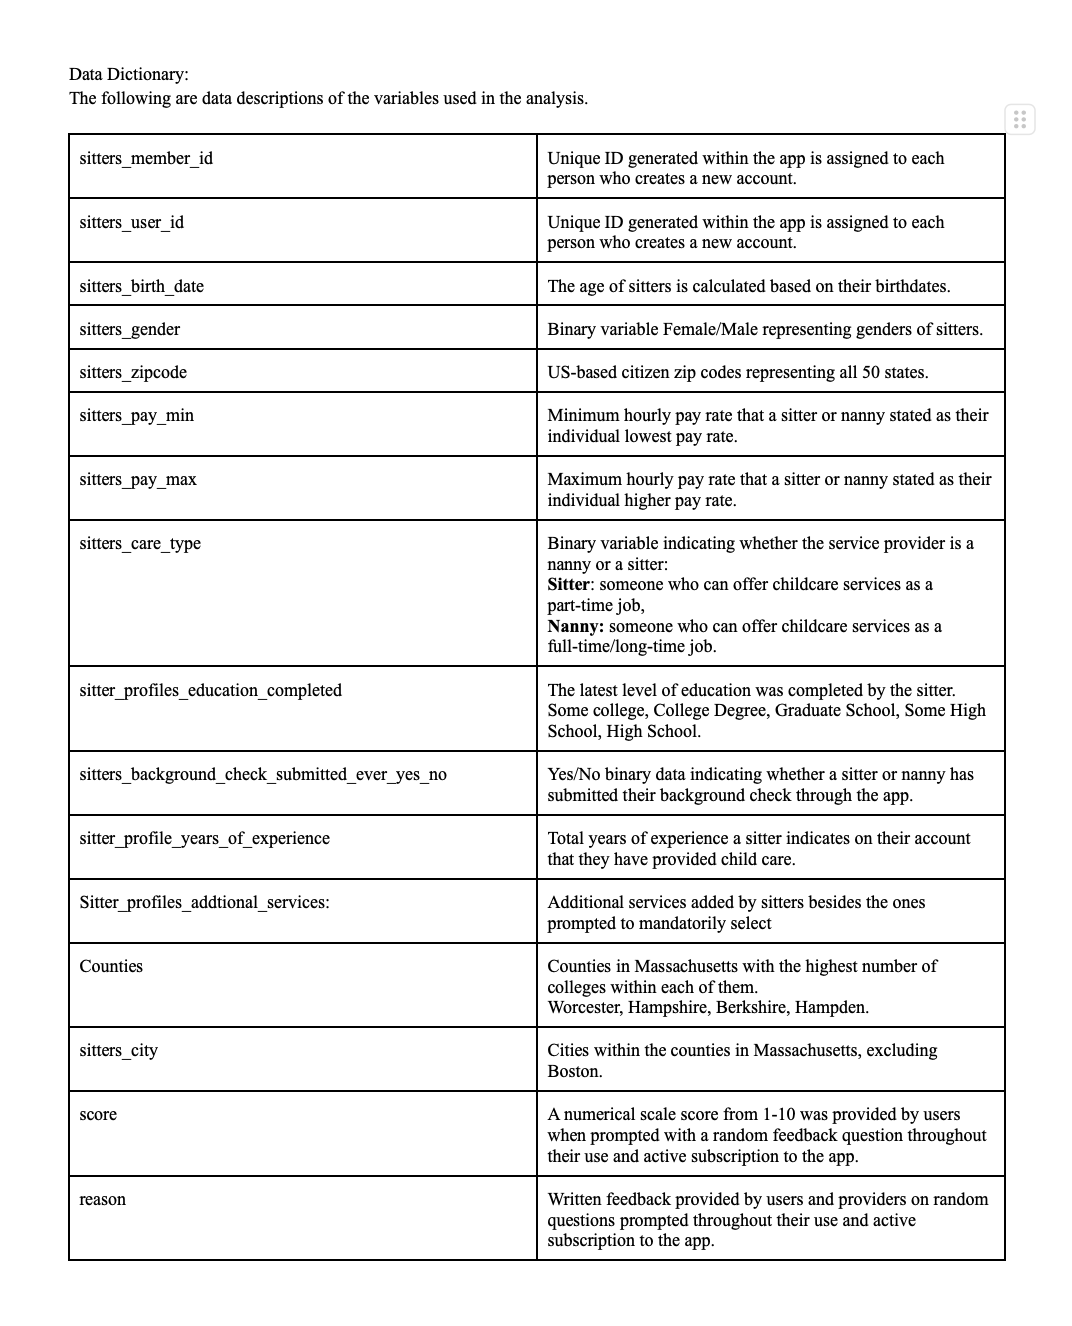
\includegraphics{IMAGES/data_dictionary.png}
\caption{Caption for the image}
\end{figure}

\begin{figure}
\centering
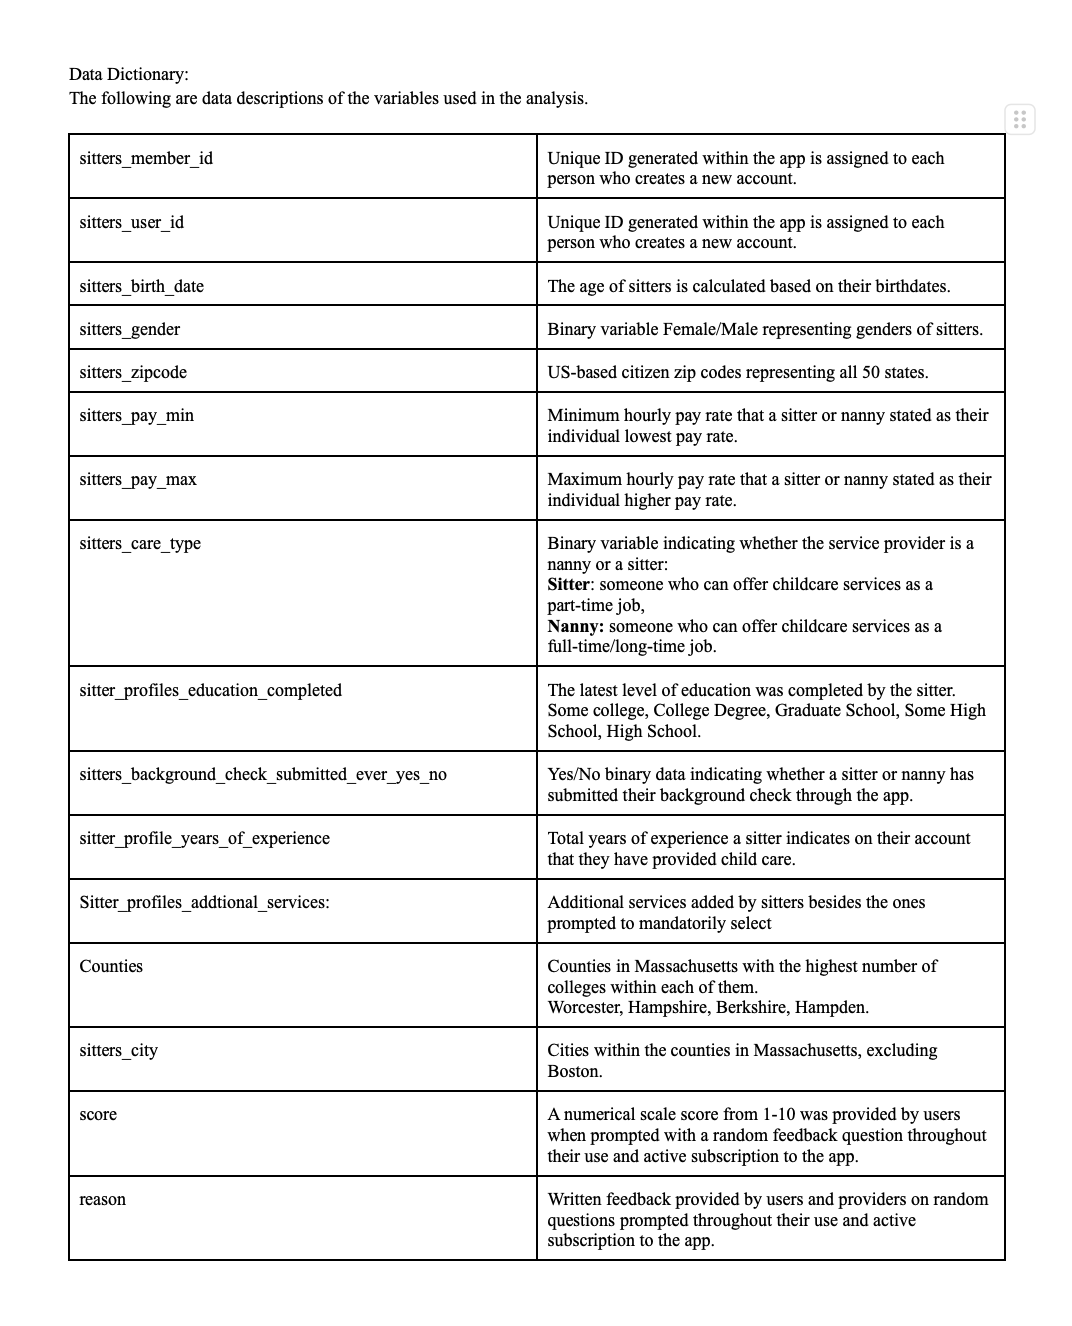
\includegraphics{IMAGES/data_dictionary.png}
\caption{Caption for the image}
\end{figure}

\hypertarget{introduction}{%
\section{Introduction}\label{introduction}}

This template demonstrates some of the basic latex you'll need to know
to create a ASA article.

\section{Verifications}
\label{sec:verify}

This section will be just long enough to illustrate what a full page of
text looks like, for margins and spacing.

\hypertarget{company-background}{%
\subsubsection{\texorpdfstring{\textbf{Company
Background}}{Company Background}}\label{company-background}}

Sittercity, founded in 2001, stands as a pioneer in the online
caregiving service industry. The platform focuses on connecting families
with a broad network of babysitters, nannies, pet sitters, senior care
providers, and tutors. The user-friendly interface allows parents to
search for caregivers based on various criteria, including location,
experience, and specific skills. In the course of its two-decade
existence, the company has evolved by incorporating advanced
technologies like background checks and enhanced matching algorithms,
ensuring safety and reliability. Sittercity's impact is significant,
modernizing the way families find and secure trusted care for their
loved ones, establishing it as a notable entity in the caregiving
industry. However, the company has faced controversies and customer
complaints, particularly related to billing practices and customer
service.

\hypertarget{introduction-1}{%
\subsubsection{\texorpdfstring{\textbf{Introduction}}{Introduction}}\label{introduction-1}}

In 2020, amidst the COVID-19 pandemic, Sittercity observed a significant
decline in parent subscriptions, while sitters' interest steadily rose.
Building on this discovery, the Smith College Sitter Team (SCST) further
investigated the discrepancy in parental subscription declines through
the internal Sittercity database and external customer reviews of the
company.

Our research revealed an increase in parents working from home due to
the pandemic and preferring the convenience that comes with a
babysitter/nanny coming to their home over a childcare center. This
choice alleviates the concern of integrating a school schedule into
their already busy routines. Additionally, we identified customer
concerns related to the company's trust and safety, and the cost of
Sittercity's background check process, as some of the main factors
contributing to parents canceling their subscriptions.

SCST suggests the introduction of a ``Sittercity x College Collab''
initiative, designed to attract more college students as potential
sitters. The envisioned outcome is an increase in parent subscriptions.
This proposal is founded on detailed findings, which will be further
elaborated in the subsequent sections of this memo.

\begin{enumerate}
\def\labelenumi{\arabic{enumi}.}
\item
  Sitters with some level of education beyond high school are found to
  be more desirable by parents:

  a. College-aged sitters of 18-24, can provide additional special
  skills at a higher rate in comparison to any other age range.\\
\item
  Eliminate Background Check Costs for parents:

  a. According to the Institute for Higher Education Policy, 72\% of
  institutions require applicants to disclose their criminal history and
  conduct student background checks.

  b. Currently, parents and sitters have to pay either: 20, 24, or 60
  dollars for a background check alone, and for parents they have to pay
  additionally a sitters pay rate. Having a college sitter eliminates
  this additional cost as the background check has already been done by
  their school.
\item
  Increase in Trust and safety from subscribed parents:\\
  \strut \\

  \begin{enumerate}
  \def\labelenumii{\alph{enumii}.}
  \tightlist
  \item
    Adding the college verification login ensures that a parent is
    getting a sitter from the accredited college they claim to be from
    and adds validity. Currently, Sittercity doesn't conduct any form of
    verification on a sitter's certifications or background unless paid
    for, however the added college login would add a layer of trust in
    Sittercity from parents.
  \end{enumerate}
\end{enumerate}

\hypertarget{data}{%
\section{\texorpdfstring{\textbf{Data}}{Data}}\label{data}}

There were three main data sets provided by Sittercity for the capstone
analysis: General Information of Sitters, Rating Information of Sitters,
and Feedback data from both providers of services and parents.

\emph{Notes:} Boston City was excluded from the cities within counties
in MA due to its already existing popularity within the app. The data
provided for analysis is the 10\% of data randomly generated and
extracted from a bigger data set. The data used only contains years
after the pandemic, 2020. This decision was made since during the
pandemic the services were discouraged due to many parents and children
staying at home and the lack of necessity for sitters. A total of 205
observations were left within the dataset once all filters were applied.

\hypertarget{methods}{%
\section{Methods}\label{methods}}

In order to supplement our proposal, pitching for the incorporation of a
College Student component on the Sittercity platform, we conducted a
comprehensive research initiative comprising both market research and
data analysis. Our objective was to not only understand the current
landscape of Sittercity but also to provide a data-driven foundation for
our proposed enhancements.

\hypertarget{market-research}{%
\subsubsection{Market Research}\label{market-research}}

\begin{enumerate}
\def\labelenumi{\arabic{enumi}.}
\item
  Unbiased Exploration:

  We started our research by obtaining an unbiased perspective on
  Sittercity. Utilizing reliable research sites, we gathered information
  to comprehend Sittercity's reputation, user interface, and overall
  user experience. This approach was crucial in identifying areas of
  improvement without any preconceived notions.
\item
  Immersive Platform Experience:

  To gain firsthand insights, we actively engaged with the Sittercity
  platform. We created decoy accounts, both from the perspective of a
  guardian and a potential sitter, immersing ourselves in the user
  experience. This hands-on approach allowed us to identify pain points
  and envision improvements from the user's standpoint.
\end{enumerate}

\hypertarget{data-analysis}{%
\subsubsection{Data Analysis}\label{data-analysis}}

\begin{enumerate}
\def\labelenumi{\arabic{enumi}.}
\item
  \textbf{Demographic Analysis}

  Leveraging existing data provided by Sittercity, we conducted a
  thorough demographic analysis focusing on both sitters and guardians.
  Our analysis included geographical locations, educational backgrounds,
  and user reviews to understand the current user base and their
  experiences with the platform.
\item
  \textbf{Massachusetts Focus}

  Recognizing the concentration of colleges and universities in
  Massachusetts, we honed in on this state for a more in-depth analysis,
  using it as a case study to support our argument for the introduction
  of a college student component. We looked into educational levels,
  locations, and levels of experience to identify the potential for a
  pool of reliable and capable college sitters in the Massachusetts
  area.
\item
  \textbf{Customer Reviews}

  As per our data analysis, we understand that customer feedback is
  invaluable, especially when implementing changes. We analyzed customer
  reviews to gauge satisfaction levels, identify recurring concerns, and
  highlight positive aspects of the platform. This qualitative data
  provided a nuanced understanding of user experiences, allowing us to
  align our proposed enhancements with user expectations.

  Our market research and data analysis yielded compelling results.
  Specifically, in Massachusetts, the abundance of college and
  university students presents a significant opportunity for the
  integration of a College Student component of Sittercity. Customer
  reviews, both positive and negative, guided us in identifying areas
  that require immediate attention and improvement. Overall, our
  holistic approach to market research and data analysis formed a robust
  foundation for our proposal.
\end{enumerate}

\hypertarget{results}{%
\section{\texorpdfstring{\textbf{Results}}{Results}}\label{results}}

In keeping with our proposed business idea, certain variables were
prioritized to deliver efficient supporting insights. To demonstrate
that the new business model could be relevant to the future of
Sittercity, we chose to focus on those sitters located in Massachusetts
broken down by county, excluding Boston only, due to the popularity of
the app in the city, we decided to focus on other cities within counties
with potential to be exploited taking into account the number of
colleges surrounding these areas.

\emph{Geographical data}: The top three counties in MA with the most
sitters represented are Hampshire, Berkshire, and Hampden.

(picture goes here)

\emph{Age range}: We deliberately decided to make five different
categories of age range to target our group of college students, since a
traditional college student would fit within the category of 18--24
years old. From the data provided, we can see that 42\% of our providers
are within that category range, which supports our idea that people
within this age range are more likely to sign up. This can be because
many of these are individuals looking for a part-time job while studying
throughout the academic year.

(picture goes here)

\emph{Level of Education}: Since Sittercity also asks for the level of
education of the service providers, we were also interested in finding
out whether most of these sitters were at college or had some type of
college instructions as their qualification. More than 45\% of sitters
signaled to either have a college degree or have some type of college
education, which we assume to refer to someone who is still in the
process of getting a degree or has completed their education.

(picture goes here)

\emph{Years of Experience}: The data also showcases that the vast
majority of sitters' years of experience range from 0--10 years,
emphasizing 0--5 years. This is another example of how the experience
that could be brought to SitterCity can be from students who have had
experience working in settings where childcare was required.

(picture goes here )

\emph{Rating Scores}: We could not represent this fact due to many
missing values. Overall, it seemed that sitters within the age range of
18-24 do not get as many ratings as other people within other age
ranges.

\emph{Hourly Pay Rate}:Another key factor of interest to our business
proposal and data analysis was looking at the hourly minimum pay rate
established by sitters in Massachusetts counties. This was to determine
whether we could advertise signing up as a sitter as a better option
than, for example, working an on-campus job with a minimum wage pay rate
of \$15 per hour. Most sitters with 0 to 8 years of experience ask and
get paid a minimum of \$18 or more. We can then conclude that a student
could make more work as a sitter for an average of 10 hours than working
on campus, or if taken as extra hours, this could also still be
beneficial enough for them to acquire a membership within the app.

(picture goes here)

\emph{Average Compensation of Sitters in MA based on Years of Experience
and Level of Education Completed}:

(picutre goes here)

note: Outliers were filtered in both dependent and independent
variables. Years of Experience = 40 Mean Pay Rate = 60

Through a regression model, we were interested in understanding whether
there were any significant differences or relationships between the
minimum pay rate and sitters' college years of experience. To summarize,
we wanted to answer the following question:

H0: Babysitters' minimum pay rate is higher based on their years of
experience. H1: Babysitters minimum pay rate is not higher based on
their years of experience.

\textbf{\emph{Do sitters get paid more based on their years of
experience or their level of education?}}

For people with only `Some High School Degree', we can observe that
their average pay rate starts very high, more than \$18, yet as years
pass by, the amount of money they get paid decreases, meaning that
although they gain more experience in the field, their missing higher
education, does lower their opportunity of a higher pay rate. For those
with a High School Degree only, the minimum pay rate starts pretty low
and gets higher as more years of experience are added, one suggestion
was that this occurs because people without a continuation of their
higher studies make their sitter job their full-time employment.

On the contrary, for those with some college education or a degree past
the undergraduate level, we can observe that although their minimum pay
rate is higher at 0 years of experience, the rate keeps increasing as
they start acquiring more years of experience. This tells us that years
of experience can help increase the pay rate asked by sitters, yet it
will be more significant for those with a college degree education,
which is our target group of people.

\emph{Special Skills within the age range 18-24}:

Times have changed and so have necessities. Due to the new remote
working environment brought about after the COVID-19 pandemic, most
parents are now at home and only need babysitting for special occasions
or to help their children with specific needs. Those sitters within the
age range of 18-24 and 25-34 are best suited with skills such as helping
with homework (tutoring), being certified for CPR and First Aid (could
be learned in college), meal preparation, and laundry, compared to those
other age ranges. The reason behind this is that when in a college
environment, a student can easily get access to these certifications
while also getting experience in different subject areas and abilities
that living in college requires someone to develop.

(picture goes here)

Text Mining Analysis on Feedback ``Reason'' for Score given data:
Sittercity, the app, randomly prompts its users in a question box to
rate their service and give written feedback on the app throughout their
time as users and when quitting the subscription. Data mining was used
to first filter the scores given, where from 0-5 it is considered
``Positive Feedback'' and 6-10 ``Negative Feedback''. Once this filter
was performed, a world cloud was built. The wordclouds can be found in
the appendix.

\emph{Positive Feedback}: Overall, patterns found can tell that users
like the easiness of use of the app, its helpfulness, and that both pay
and the wide variety of range of sitters have provided users a good
experience that would make them recommend the app to other people.

\emph{Negative Feedback}: On the other hand, first, the negative
feedback tells that the main issue around dissatisfaction with the
service is the unavailability of sitters within specific mile ranges,
second the fact that a background check needs to be paid for by parents
can also become an obstacle for people to use the service, and lastly
the ineffectiveness of communication and to get to have the actual
sitter perform their job from the first message contact to real life.

\hypertarget{next-steps}{%
\subsubsection{\texorpdfstring{\uline{\textbf{Next
Steps:}}}{Next Steps:}}\label{next-steps}}

A dedicated tab will be provided for college students to register.
During the sign-up process, students will encounter the familiar
registration page, with a strong encouragement to register using their
official school email addresses. Following registration, students will
receive a verification email prompting them to confirm their email and
verify their identity. Upon successful registration, they can log in
using their school credentials, triggering a two-factor authentication
process facilitated by the university's IT service administrator. It's
important to note that the two-factor authentication process is a
separate procedure managed by the university IT services.

After completing the verification process, the sitter's profile will be
marked with a green checkmark, signifying a verified college student
sitter. This streamlined verification is facilitated by the prior
background check conducted during their enrollment through the
institution. This will allow parents to promptly recognize and ensure
the credibility of verified sitters.

If parents desire an additional layer of security and opt for a
background check, they can make that request, which college students can
swiftly and easily fulfill. This is possible because specific
departments within their college campuses provide the required
documentation upon request.

Students will sign up at a reduced cost and this will give them access
to the badge and prioritization in the services offered search results.
However, students will be offered a free one-month trial first. Once
they realize they can make more of their time through the flexibility of
hours offered and set a higher minimum pay rate, then they will choose
to stay in the app and pay for the monthly subscription.~

(picture goes here)

\hypertarget{parental-benefits}{%
\subsubsection{\texorpdfstring{\textbf{Parental
Benefits}}{Parental Benefits}}\label{parental-benefits}}

\textbf{Expanded Service Variety:}

Parents will benefit from a broader array of services beyond traditional
babysitting. College Students may offer additional services such as
language practice, physical activities, or music lessons. This enhances
the options available for parents, catering to a diverse set of needs.

\textbf{Reliability and Trust:}

The collaboration between SitterCity and colleges introduces a new batch
of subscribers, and a potentially more reliable and trustworthy pool of
sitters. This can instill confidence in parents, as the platform
leverages the credibility of college communities and their associated
values.

\textbf{Geographic Coverage Assurance:}

Addressing concerns raised by parents in certain areas, the targeted
coverage around college campuses aims to ensure that premium users can
find adequate service providers. This strategic approach contributes to
a more reliable and widespread availability of sitters in locations
where parents often seek childcare services.

\textbf{Cost-Efficiency:}

The potential reduction in marketing expenses coupled with the increase
in subscribers from college communities indirectly benefits parents.
Additionally, as the platform grows, operational costs may be better
distributed, potentially resulting in cost-effective services for
parents.

\hypertarget{student-perks}{%
\subsubsection{\texorpdfstring{\textbf{Student
Perks}}{Student Perks}}\label{student-perks}}

Students can sign up at a reduced cost and enjoy a complimentary
one-month trial. As they discover the advantages of the SitterCity
student account, they may opt to continue using it and subscribe to the
monthly plan.~

Students subscribing to the service can access a range of perks, like
discounts at local stores and additional subscriptions such as Hulu and
Spotify. They also have the opportunity to become Sitter City brand
ambassadors, where they can organize on-campus events and workshops,
promoting the app within the community.~

\hypertarget{business-incentives}{%
\subsubsection{\texorpdfstring{\textbf{Business
Incentives}}{Business Incentives}}\label{business-incentives}}

\textbf{Increase Subscriber Base}

The collaboration between SitterCity and colleges has the potential to
significantly boost the number of subscribers.~

\textbf{Enhance Parent Services}

With a diverse pool of sitters offering various talents, the platform
becomes a reliable resource for parents seeking childcare with unique
and supplementary services.

\textbf{Targeted Location Coverage}

Recognizing the widespread presence of colleges across states, tapping
into college student communities ensures a broad geographic coverage.
This strategic approach addresses feedback about insufficient service
providers in specific areas, especially where premium users seek
sitters. By focusing on zones around college campuses, this
collaboration aims to alleviate this issue.

\textbf{Revenue Growth}

The anticipated influx of subscribers from college student communities
is poised to drive a significant increase in SitterCity's revenue. This
growth is expected to be accompanied by a reduction in marketing and
advertising expenses. Additionally, this collaboration strengthens the
platform's trustworthiness, positioning it as a reliable choice for
finding service providers, addressing existing weaknesses in comparison
to competitors.

\hypertarget{conclusion}{%
\section{Conclusion}\label{conclusion}}

To summarize our capstone, we can start by stating that the goal of this
project was open-ended from the very beginning, Thus, we came up with a
business proposal of interest for our data sponsor, Sittercity, by
conducting an extensive exploratory data analysis combined with our
experiences as college students based in Massachusetts, specifically
within the 5-college community. This business plan was intended to
counter the decline in premium subscribers and to realign Sittercity
towards its foundational objective of serving as a platform for offering
childcare services. Once we found out that the data provided by
Sittercity matched the skills and demographics of most college students,
we proposed a new subscription for college students only at a lower rate
than what the actual premium subscribers pay now along with external
research that supported the effectiveness of the idea.~

\hypertarget{limitations}{%
\subsubsection{\texorpdfstring{\textbf{Limitations}}{Limitations}}\label{limitations}}

The main limitation of this business case study is the randomization and
small sample size of the data compared to the original sample size
provided to us. Due to us only extracting 10\% of the data, we were left
with a sample size that was not as significant and therefore not
representative of the entire population of Sittercity subscribers.
Similarly, Massachusetts as a singular state is not representative of
all states of the US, therefore an assumption that the business case
presented within MA could work in other states is indefinite. Lastly, we
chose to focus on efforts related to the sitters, and we did not analyze
much data related to the other types of service providers nor the
parents or service users.~

\hypertarget{future-applications}{%
\subsubsection{\texorpdfstring{\textbf{Future
applications}}{Future applications}}\label{future-applications}}

Analyzing the data with a full dataset divided by states all across the
US would provide a better understanding of the general profile of the
most popular sitters. Additionally, conducting a text analysis using the
feedback provided to the app would be beneficial to identifying
targeting points from specific communities in order to effectively come
up with strategies that could improve the service.~

The next steps for this business proposal would be to conduct a test
group within one of the suggested college communities where the idea is
implemented, followed by a careful analysis of the profits and revenues
made as well as the effectiveness of the service app for both sitters
and providers of the services. Additionally, it would be beneficial to
conduct a pilot group for a minimum of a year, including winter and
summer breaks to also have an overview of the results throughout the
fluctuation of the school year. We some business schools would be prime
candidates for collaborating with this project.

\bibliographystyle{plain}
\bibliography{}



\end{document}
